\documentclass[a4paper,10pt]{article}

% Packages
\usepackage[utf8]{inputenc}
\usepackage[frenchb]{babel}
\usepackage{graphicx}
\usepackage{url}
\usepackage{hyperref}
\usepackage{a4wide}
\usepackage{amsmath}
\usepackage{verbatim}
\usepackage{eurosym}
\usepackage{array}
\usepackage{../clrscode3epg}
\renewcommand{\labelenumi}{(\alph{enumi})}

% Style
\parskip=\smallskipamount

% En-têtes
\title{
    \textbf{Structures de données et algorithmes}\\
    Répétition 9: Graphes
}

\author{Gilles \textsc{Louppe} -- \url{http://www.montefiore.ulg.ac.be/~glouppe}}
\date{10 mai 2013}

% Corps
\begin{document}
\maketitle


\section*{Exercice 1}

\begin{enumerate}
\item A quoi ressemble un graphe dont tous les sommets sont de degré 1 exactement?
\item A quoi ressemble un graphe dont tous les sommets sont de degré 2 exactement?
\item Si un graphe non orienté possède $n$ sommets, tous de degré $d$, combien comporte t-il d'arêtes?
\end{enumerate}

\section*{Exercice 2}

Soit un graphe $G$ dont $A$ est la matrice d'adjacence.

\begin{enumerate}
\item Caractériser le graphe $G'$ dont $A^T$ est la matrice d'adjacence.
\item Quelle interprétation peut-on faire du produit $AA$?
\item Quelle interprétation peut-on faire du produit $A^k$?
\end{enumerate}

\section*{Exercice 3}

Pour les cas suivants, est-il plus approprié d'utiliser un graphe implémenté par une liste d'adjacences ou par une matrice d'adjacence? Justifier.

\begin{enumerate}
\item Le graphe possède 10000 sommets et 20000 arêtes et on souhaite minimiser l'espace mémoire utilisé.
\item Le graphe possède 10000 sommets et 2000000 arêtes et on souhaite minimiser l'espace mémoire utilisé.
\item On souhaite déterminer le plus rapidement possible si deux sommets sont adjacents, peu importe l'espace mémoire requis.
\end{enumerate}

\section*{Exercice 4}

Illustrer graphiquement l'exécution de l'algorithme de Dijkstra sur le graphe de la Figure 1. On souhaite trouver tous les plus courts chemins à partir du sommet BWI.

\begin{figure}
    \center
    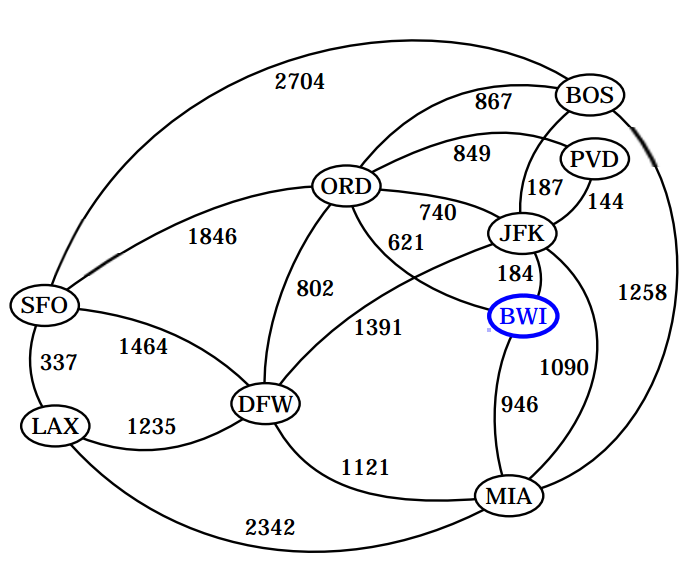
\includegraphics[scale=0.5]{graphe.png}
    \caption{Graphe}
\end{figure}

\section*{Exercice 5}

Dans certaines applications (les réseaux notamment), une architecture de graphes
est utilisée et un des noeuds joue souvent un rôle spécial par rapport aux
autres (e.g., un serveur de fichiers au sein d'un réseau d'ordinateurs). Pour
obtenir des performances optimales, on souhaiterait déterminer ce noeud comme le
"centre" du graphe. Pour cela, on définit, étant donné un graphe $G$ et un noeud
$v$, l'excentricité de $v$ comme la longueur du plus long des plus courts
chemins entre $v$ et tous les autres noeuds de $G$. Le centre de $G$ est défini
comme le noeud d'excentricité minimale.

\begin{enumerate}
\item Proposer un algorithme pour calculer le centre d'un graphe $G$.
\item Quelle est sa complexité si $G$ est implémenté par une liste d'adjacences?
\item  Quelle est sa complexité si $G$ est implémenté par une matrice d'adjacence?
\end{enumerate}

\section*{Exercice 6}

Les échelles de mots sont un jeu (inventé par Lewis Carroll) où l’on doit
passer d’un mot à un autre en utilisant des mots intermédiaires, et où à chaque étape, une
seule lettre est enlevée, ajoutée ou remplacée par une autre, les autres restant identiques
et dans la même position. Toutes les formes grammaticales sont permises. On se restreint
ici aux mots de même longueur.

\begin{enumerate}
\item Passer (en anglais) de LESS à MORE.
\item Proposer un algorithme pour résoudre ce problème de façon générique, étant donné
une liste de mots de $n$ lettres.
\end{enumerate}

\section*{Exercice 7}

Huit îles se trouvent sur un lac. Le gouvernement local souhaite construire
sept ponts pour les relier, de sorte qu'on puisse rejoindre n'importe quelle
île depuis n'importe quelle autre en traversant un ou plusieurs ponts. Le
coût de construction d'un pont est proportionnel à sa longueur. Sachant
que la table ci-dessous énumère les distances entre chaque île, quels sont les
ponts à construire pour minimiser le coût total de construction?

\begin{verbatim}
        1       2       3       4       5       6       7       8
1       -       240     210     340     280     200     345     120
2       -       -       265     175     215     180     185     155
3       -       -       -       260     115     350     435     195
4       -       -       -       -       160     330     295     230
5       -       -       -       -       -       360     400     170
6       -       -       -       -       -       -       175     250
7       -       -       -       -       -       -       -       305
8       -       -       -       -       -       -       -       -
\end{verbatim}

\end{document}
